\documentclass{article} % For LaTeX2e
\usepackage{nips14submit_e,times}
\usepackage{amsmath}
\usepackage{amsthm}
\usepackage{amssymb}
\usepackage{mathtools}
\usepackage{hyperref}
\usepackage{url}
\usepackage{algorithm}
\usepackage[noend]{algpseudocode}
%\documentstyle[nips14submit_09,times,art10]{article} % For LaTeX 2.09

\usepackage{bbm}
\usepackage{graphicx}
\usepackage{caption}
\usepackage{subcaption}
\usepackage{MnSymbol}

\def\eQb#1\eQe{\begin{eqnarray*}#1\end{eqnarray*}}
\def\eQnb#1\eQne{\begin{eqnarray}#1\end{eqnarray}}
\providecommand{\e}[1]{\ensuremath{\times 10^{#1}}}
\providecommand{\pb}[0]{\pagebreak}
\DeclarePairedDelimiter\ceil{\lceil}{\rceil}
\DeclarePairedDelimiter\floor{\lfloor}{\rfloor}

\newcommand{\E}{\mathrm{E}}
\newcommand{\Var}{\mathrm{Var}}
\newcommand{\Cov}{\mathrm{Cov}}

\def\Qb#1\Qe{\begin{question}#1\end{question}}
\def\Sb#1\Se{\begin{solution}#1\end{solution}}

\newenvironment{claim}[1]{\par\noindent\underline{Claim:}\space#1}{}
\newtheoremstyle{quest}{\topsep}{\topsep}{}{}{\bfseries}{}{ }{\thmname{#1}\thmnote{ #3}.}
\theoremstyle{quest}
\newtheorem*{definition}{Definition}
\newtheorem*{theorem}{Theorem}
\newtheorem*{lemma}{Lemma}
\newtheorem*{question}{Question}
\newtheorem*{preposition}{Preposition}
\newtheorem*{exercise}{Exercise}
\newtheorem*{challengeproblem}{Challenge Problem}
\newtheorem*{solution}{Solution}
\newtheorem*{remark}{Remark}
\usepackage{verbatimbox}
\usepackage{listings}
\usepackage{mathrsfs}
\title{ProbLimI: \\
Problem Set II}


\author{
Youngduck Choi \\
CIMS \\
New York University\\
\texttt{yc1104@nyu.edu} \\
}


% The \author macro works with any number of authors. There are two commands
% used to separate the names and addresses of multiple authors: \And and \AND.
%
% Using \And between authors leaves it to \LaTeX{} to determine where to break
% the lines. Using \AND forces a linebreak at that point. So, if \LaTeX{}
% puts 3 of 4 authors names on the first line, and the last on the second
% line, try using \AND instead of \And before the third author name.

\newcommand{\fix}{\marginpar{FIX}}
\newcommand{\new}{\marginpar{NEW}}

\nipsfinalcopy % Uncomment for camera-ready version

\begin{document}


\maketitle

\begin{abstract}
This work contains solutions to the exercises of the problem set I. The
chosen problems are 1,2, and 4.
\end{abstract}

\bigskip

\begin{question}[1]
\hfill
\begin{figure}[h!]
  \centering
    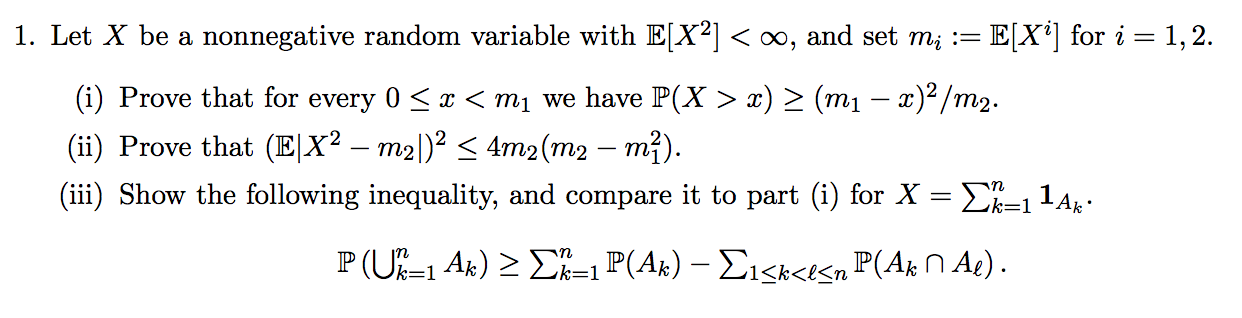
\includegraphics[width=0.7\textwidth]{problim-e2-p1.png}
\end{figure}
\end{question}
\begin{solution} \hfill \\
\end{solution}

\newpage

\begin{question}[2]
\hfill
\begin{figure}[h!]
  \centering
    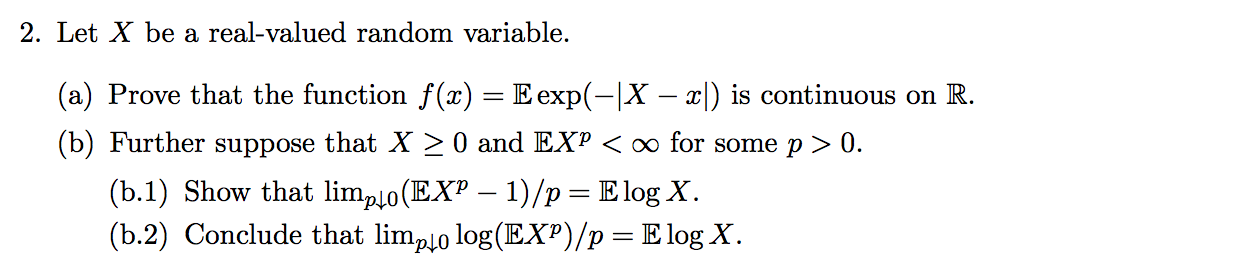
\includegraphics[width=0.7\textwidth]{problim-e2-p2.png}
\end{figure}
\end{question}
\begin{solution} \hfill \\

\end{solution}

\newpage

\begin{question}[3]
\hfill
\begin{figure}[h!]
  \centering
    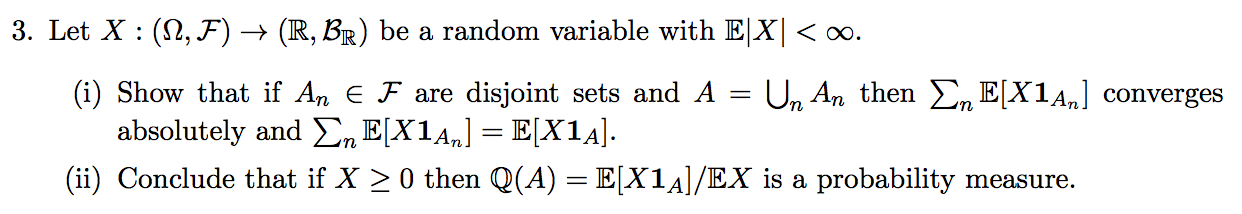
\includegraphics[width=0.7\textwidth]{problim-e2-p3.png}
\end{figure}
\end{question}
\begin{solution} \hfill \\
We first show the case for non-negative, simple functions. Let $X$ be simple, such that
\eQb
X &=& \sum_{k=1}^{l} a_k \mathbbm{1}_{E_k},
\eQe
where $a_k \in \mathbb{R}$ for $k = 1,...,l$ and $E_k \in \mathscr{F}$ 
with $\bigcupdot_{k=1}^{l} E_k = \Omega$. With linearity of expectation,
\eQb
\mathbb{E}[X\mathbbm{1}_{A}] &=& \mathbb{E}[\sum_{k=1}^{l} a_k \mathbbm{1}_{E_k}
\mathbbm{1}_{A}] 
= \sum_{k=1}^{l} a_k\mathbb{E}[\mathbbm{1}_{E_k} \mathbbm{1}_{A}] \\
&=& \sum_{k=1}^{l} a_k\mathbb{E}[\mathbbm{1}_{E_k \cap A}] 
= \sum_{k=1}^{l} a_k \mathbb{P}(E_k \cap A).
\eQe  
Similarly,
\eQb
\mathbb{E}[X\mathbbm{1}_{A_n}] &=& \sum_{k=1}^{l} a_k\mathbb{P}(E_k \cap A_n) 
\eQe
for each $n \geq 1$. Then, it follows that, for all $m \geq 1$,
\eQb
\sum_{n=1}^{m} |\mathbb{E}[X\mathbbm{1}_{A_n}]| &=& \sum_{n=1}^{m} \sum_{k=1}^{l} 
a_k \mathbb{P}(E_k \cap A_n) \\
&=& \sum_{k=1}^{l} a_k \mathbb{P}(E_k \cap \bigcup_{m\geq n} A_n), \\
\eQe
where the equality holds by disjointness of $\{A_n\}$. Since $\bigcup_n A_n = A$,
we can exploit continuity of probability and obtain 
\eQb
\sum_{n} |\mathbb{E}[X\mathbbm{1}_{A_n}]| &=& \lim_{m \to \infty} \sum_{k=1}^{l} a_k
\mathbb{P}(E_k \cap \bigcup_{m \geq n} A_n) \\
&=& \sum_{k=1}^{l} a_k \lim_{m \to \infty} \mathbb{P}(E_n \cap \bigcup_{m \geq n}
A_n) = \sum_{k=1}^{l} a_k \mathbb{P}(E_n \cap A) = \mathbb{E}[X\mathbbm{1}_A].
\eQe
Hence, we have shown that for $X$ non-negative and simple, $\sum_{n} 
\mathbb{E}[X\mathbbm{1}_{A_n}]$ converges absolutely to $\mathbb{E}[X\mathbbm{1}_{A}]$. 

\bigskip

We now extend the case to non-negative integrable functions. 
Let $X$ be a bounded, measurable, non-negative functions. Choose $\{ \phi_k\}$
simple functions such that $\phi_k \to X$. By the previous result, 
we observe
\eQb
\sum_{n} \mathbb{E}[\phi_k \mathbbm{1}_{A_n}] = \mathbb{E}[\phi_k \mathbbm{1}_{A}] 
\>\> (*)
\eQe
for any $k \geq 1$. Since $\phi_k \to X$ uniformly, by monotone convergence theorem,
\eQb
\mathbb{E}[\phi_k \mathbbm{1}_{A}] \to \mathbb{E}[\phi_k \mathbbm{1}_{A}]
\eQe
and
\eQb
\mathbb{E}[\phi_k \mathbbm{1}_{A_n}] \to \mathbb{E}[\phi_k \mathbbm{1}_{A_n}]
\eQe
which via implies
\eQb
\sum_{n} \mathbb{E}[\phi_k \mathbbm{1}_{A_n}] \to \sum_{n} 
\mathbb{E}[\phi_k \mathbbm{1}_{A_n}].
\eQe
Combining (*) with the above limit, we see that 
$\sum_{n} 
\mathbb{E}[X\mathbbm{1}_{A_n}]$ converges absolutely and 
$\sum_{n} 
\mathbb{E}[X\mathbbm{1}_{A_n}] = \mathbb{E}[\mathbbm{1}_{A}]$ as required.
By considering the positive part and negative part, we can extend the
result to any random variable as required. 

\textbf{(ii)} Firstly, observe that
\eQb
\mathbb{Q}(\Omega) &=& \dfrac{\mathbb{E}[\mathbbm{1}_{\Omega}]}{\mathbb{E}[X]} = 
\dfrac{\mathbb{E}[X]}{\mathbb{E}[X]} = 1.
\eQe
Hence, it now suffices to show that $\mathbb{Q}$ is countably additive, but from
the discussion in $(i)$, we see
\eQb
\mathbb{Q}(\bigcup_n A_n) &=& \dfrac{\mathbb{E}[X\mathbbm{1}_{\cup_n A_n}]}{
\mathbb{E}[X]}  
= \dfrac{\sum_{n} \mathbb{E}[X\mathbbm{1}_{A_n}]}
{\mathbb{E}[X]} = \sum_n \mathbb{Q}(A_n).
\eQe
for any $\{A_n\} \subset \mathscr{F}$ that are pairwise disjoint. So,
$\mathbb{Q}$ is a probability measure, if $X \geq 0$ and we are done
\hfill $\qed$
 
\end{solution}

\newpage

\begin{question}[4]
\hfill
\begin{figure}[h!]
  \centering
    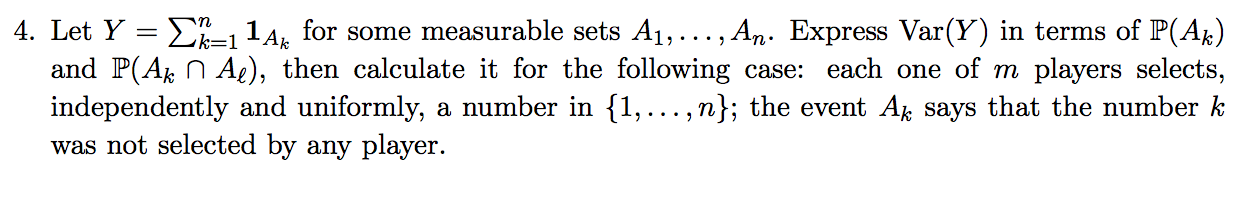
\includegraphics[width=0.7\textwidth]{problim-e2-p4.png}
\end{figure}
\end{question}
\begin{solution} \hfill \\
\end{solution}

\end{document}
